\chapter{Overview of JavaScript and V8 engine architecture}
\label{cha:overview}

Historically, JavaScript was considered an untyped language, meaning that values had no types attached to variables, either by the programmer or the compiler. All variables were of a single, unified type, and procedures called unboxing and boxing, performed before and after each operation on a variable, ensured that it was properly used on the machine code level. The complete code source was sent from the server to the browser and was parsed and executed on the fly. Without types attached to variables, all functions were polymorphic and unstable, since parameters may have carried any type of variable. To solve this problem, the source code of the function was parsed every time it was called, each time generating a machine code based on current parameters and variables in scope. This approach, called interpretation, is still present in JavaScript engines, and used whenever variables do not match set criteria of stability described later in this chapter.

This paper uses as an engine of choice V8 Crankshaft. This choice was made, because it is the only engine available at the moment which provides direct command line access, enabling the precise performance measurements of code parsing and execution, without browser context and overhead. The executable file of V8 (named d8) is compiled with consideration to the target platform.

\section{JIT compilation -- tracking variable types}
\label{sec:JIT}

As it was mentioned before, initially JavaScript was treated as an untyped language. With the release of SpiderMonkey in Firefox 3.5 in 2009, the situation changed. The first Just-In-Time compiler for JavaScript, TraceMonkey, was created. Based on the works of Prof. Dr. Michael Franz on TraceTrees \cite{Franz94code-generationon-the-fly:} JIT compiler collected all paths that the interpreter took with specific types of variables. A path could split into different methods or if statements. Whenever part of the code was executed often enough, the path was marked as hot, and the compiler optimised it for given types. If a single path was traversed with a different set of types, the compiler could generate another version of the optimised code. When the path turned out to be highly polymorphic, optimised versions were removed and the interpreter was used as a fallback.
Initial reports show speedups between 20x to 40x \cite{firefox-to-get-massive-javascript-performance-boost}.
However, trace JIT turned out to be very complicated to maintain \cite{improving-javascript-performance-with-jagermonkey} and eventually was removed from Firefox in 2011.\cite{trace-jit-removed-from-firefox}. At the time SpiderMonkey was already equipped with JagerMonkey, JIT engine based on method calls. Instead of collecting complete traces, only method calls are counted. This provides easy tracking of function parameters and variables in scope.

\begin{figure}[h!]
  \caption{JIT compiler tracking method calls}
  \label{img:jit-1}
  \centering
	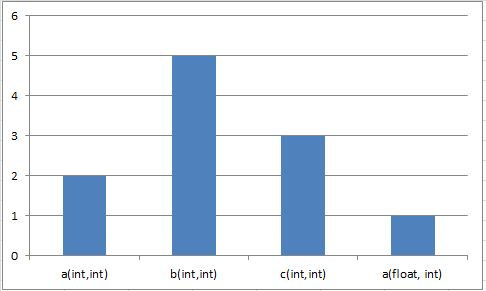
\includegraphics[width=8cm]{jit-1}
\end{figure}


\begin{figure}[h!]
  \caption{JIT compiler marking one of methods as hot and recompiling}
  \label{img:jit-2}
  \centering
	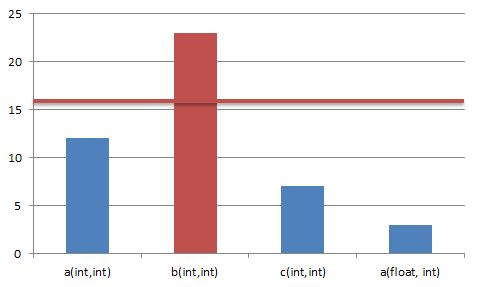
\includegraphics[width=8cm]{jit-2}
\end{figure}

This proved to be more effective and a simpler approach, which is now used in all JavaScript engines. In V8 Crankshaft, a step forward was taken, and simple methods are compiled even before any statistics on data types are collected. For compiled methods the source code is not stored. Instead, a procedure called deoptimisation is implemented. Whenever an engine detects that a compiled code does not match actual types of variables, the code is deoptimised and either optimised again to match the new, better set of variables, or kept in interpreter-friendly form.

To track these changes two debug options for V8 are available: --trace-opt and --trace-deopt.

\lstinputlisting[caption=Output from V8 debug run showing optimisation and deoptimisation,label=listing:optdeopt]{optdeopt.txt}


\section{Type inference}
\label{sec:typeference}

V8's method of optimising code before it is run relies on type inference. Based on the context of the variable its type is guessed. The generated assembler has to support cache miss -- whenever inferred type turns out to be incorrect, a new type is assigned and another JIT compilation runs. Types of variables are organised in a tree, where the Number object may store both Float or Integer, Integer may store SMI (small int), etc.

\lstinputlisting[caption=Tree of types in JavaScript,label=listing:typestree]{types.txt}

In V8 type inference is tightly connected with JIT compilation and may be tracked with the same flags: --trace-opt and --trace-deopt. 

\section{Hidden classes}
\label{sec:hiddenclasses}

JavaScript is a classless language. Object may have defined a prototype which behaves similar to base class in other langauges. However, a property may be added to an Object or its prototype at any point in runtime. To optimise such a dynamic representation, engines use the concept of hidden class. Whenever an Object is created, its hidden class is pointed to the base, empty Object representation. Then each definition of new property makes a transition on the hidden class graph, introducing hidden classes that are not yet defined, as in the following example:

\begin{figure}[h!]
  \caption{Initial shape of hidden class for Point}
  \label{img:point0}
  \centering
	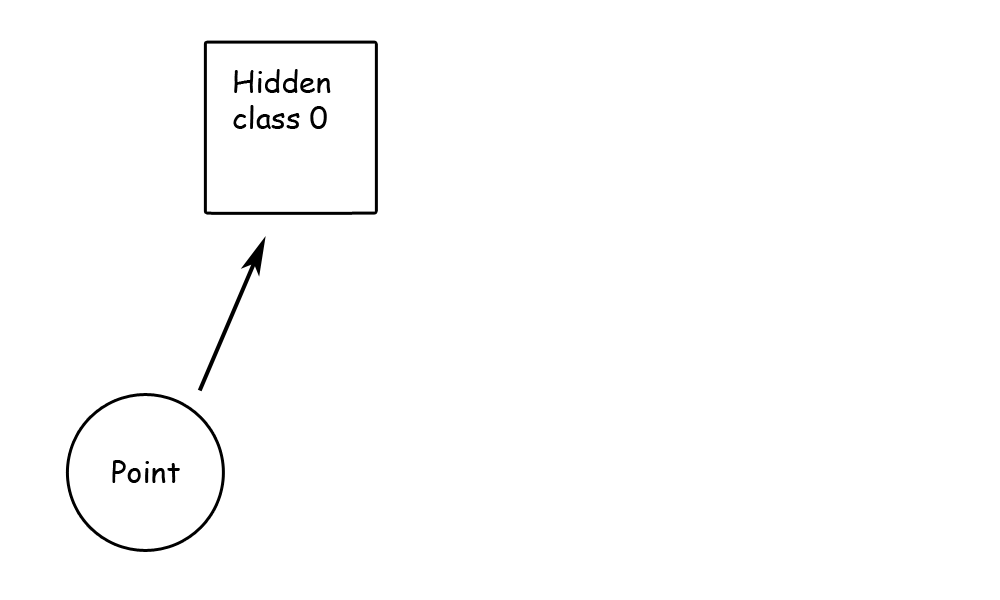
\includegraphics[width=8cm]{point0}
\end{figure}
\begin{figure}[h!]
  \caption{Shape of hidden class for Point after x property added}
  \label{img:point1}
  \centering
	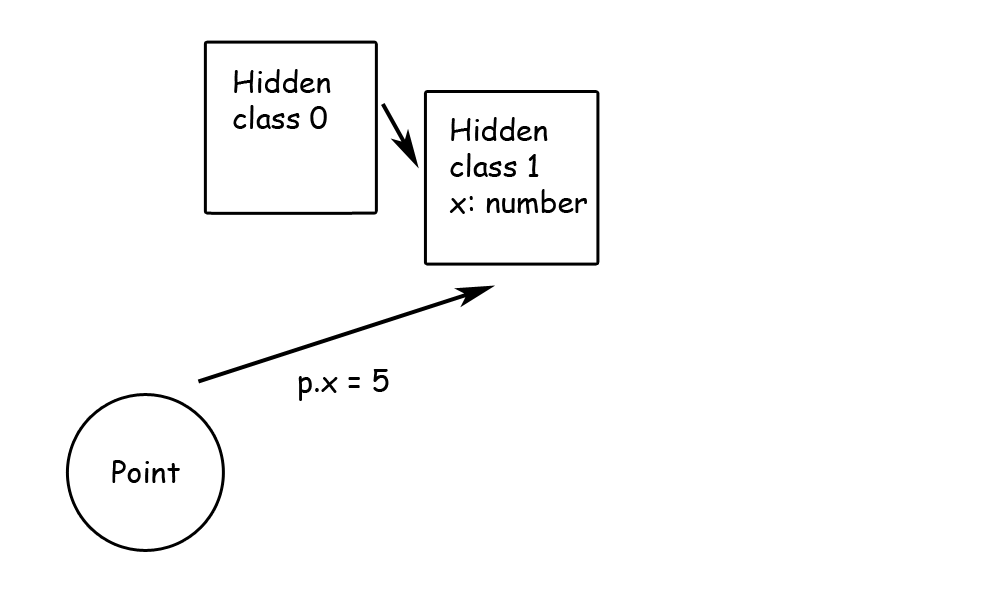
\includegraphics[width=8cm]{point1}
\end{figure}
\begin{figure}[h!]
  \caption{Shape of hidden class for Point after y property added}
  \label{img:point2}
  \centering
	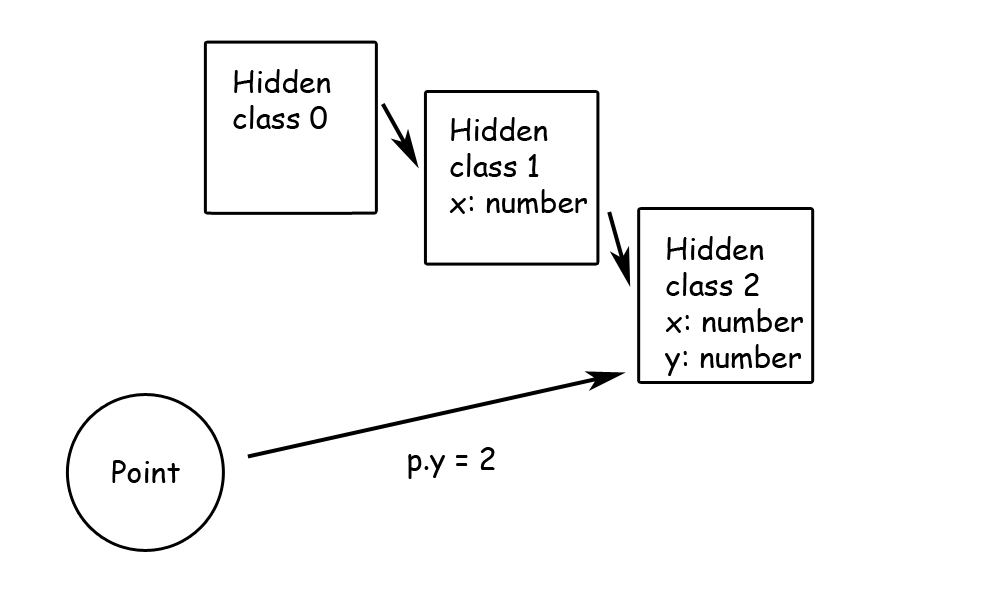
\includegraphics[width=8cm]{point2}
\end{figure}

Based on hidden class the JIT compiler optimises methods to generate an even simpler assembly code similar to the one compiled from C++. Class shape defines address offsets of Object properties. Thus, the hidden class graph is actually a tree, where one class cannot be reached in more than one way.

\begin{figure}[h!]
  \caption{Two point representations based on order of declared properties}
  \label{img:point_tree2}
  \centering
	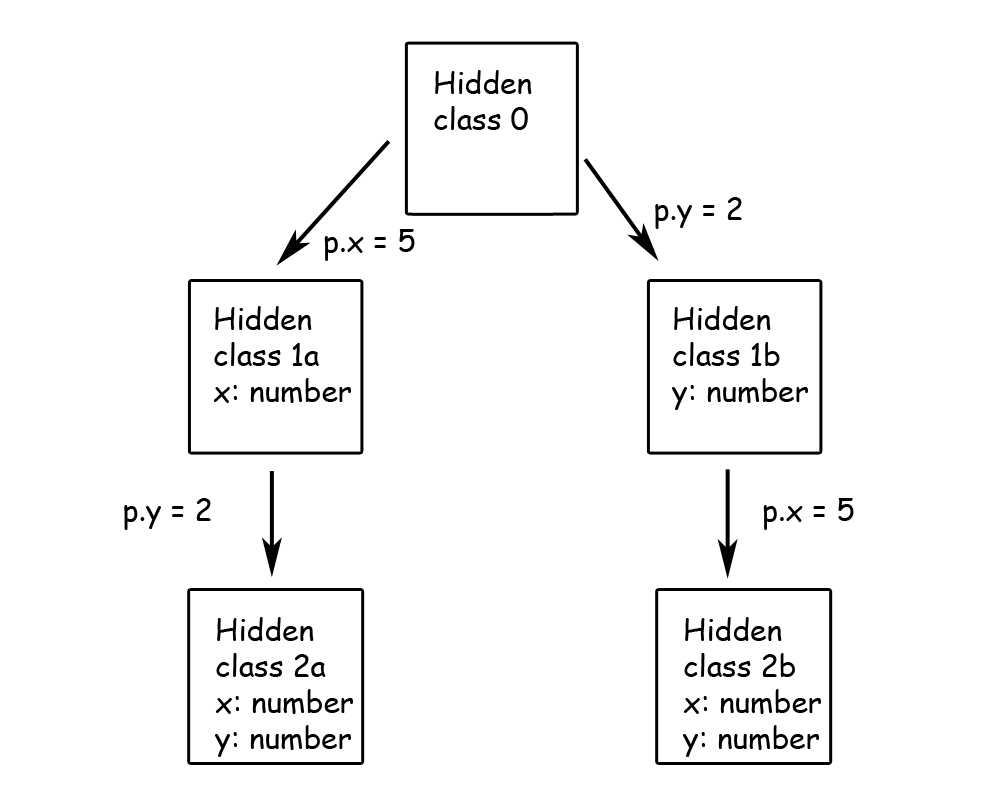
\includegraphics[width=8cm]{point_tree2}
\end{figure} 

At the moment of writing, the type of property is not tracked in hidden classes. The only exception are primitive values (see Listing \ref{listing:typestree}). In other words, storing an object in property results in the same hidden class, regardless of the hidden class of this object.

Transitions between hidden classes can be tracked in V8 using flags --trace-generalization tracking when variables are cast to a more generic type (e.g. SMI to Integer, or Integer to Number) and --trace-migration (tracking when hidden classes are migrated).

\lstinputlisting[caption=Log of migration trace in V8,label=listing:migration]{migration.txt}

\section{Garbage collection}
\label{sec:garbagecollection}

Memory in JavaScript is managed automatically. Each allocation places an object on a memory heap. The first generation of garbage collection traversed the whole tree and freed memory for all inaccessible objects. This type of deallocation is called mark-sweep and takes a long time. Since JavaScript is single-threaded, this operation blocks all other operations. To improve performance, especially in games, the incremental scavange method of garbage collection was introduced. The engine tracks the age of objects, allowing to quickly detect objects allocated temporarily (e.g. for a single frame rendered in a game). When the object is inaccessible, it is queued for deallocation, in chunks that do not cause long UI freezes.\cite{cheneys-algorithm,garbage-collection}

\lstinputlisting[caption=Log of garbage collection in V8,label=listing:gc]{gc.txt}
